\documentclass[tikz]{standalone}
\usepackage{pgfplots}
\pgfplotsset{compat=1.15}
\usepackage{mathrsfs}
\usetikzlibrary{arrows,calc}
\usepackage{tkz-euclide}
\pagestyle{empty}

\definecolor{AngleClr}{rgb}{0,0.39215686274509803,0}
\definecolor{ShapeClr}{rgb}{0.6,0.2,0}

\begin{document}

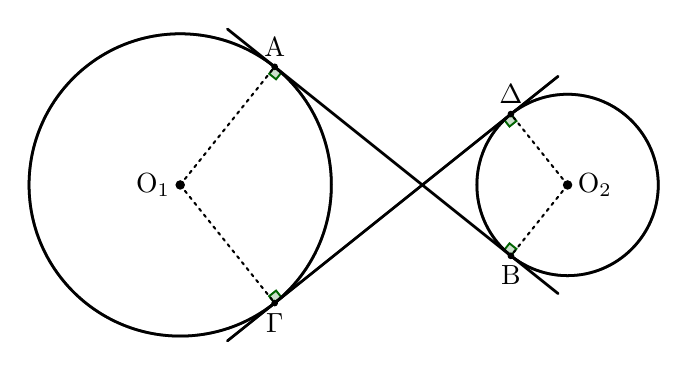
\begin{tikzpicture}[scale=.75]
\tkzSetUpLine[line width=1pt,color=black]
\tkzSetUpPoint[fill=black]

% \tkzDefPoints{0/0/O1,7/0/O2,3.5/0/A,2.5/0/B,17.5/0/P}

\tkzDefPoints{-3/2/A,1/-1.2/B,-3/-2/C,1/1.2/D}

% \tkzDefTangent[from = P](O1,A) \tkzGetPoints{TC}{TA}
% \tkzDefTangent[from = P](O2,B) \tkzGetPoints{TD}{TB}

\tkzDefLine[orthogonal=through A](A,B) \tkzGetPoint{a}
\tkzDefLine[orthogonal=through B](A,B) \tkzGetPoint{b}
\tkzDefLine[orthogonal=through C](C,D) \tkzGetPoint{c}
\tkzDefLine[orthogonal=through D](C,D) \tkzGetPoint{d}

\tkzInterLL(A,a)(C,c) \tkzGetPoint{O1}
\tkzInterLL(B,b)(D,d) \tkzGetPoint{O2}

\tkzDrawCircle[line width=1.0pt,fill=white](O1,A)
\tkzDrawCircle[line width=1.0pt,fill=white](O2,B)

\tkzMarkRightAngles[line width=0.7pt, size=.15,color=AngleClr,fill=AngleClr,fill opacity=0.2](O1,A,B O2,B,A O1,C,D O2,D,C)

\tkzDrawCircle[line width=1.0pt,color=black](O1,A)
\tkzDrawCircle[line width=1.0pt,color=black](O2,B)

\tkzDrawSegments[line width=1pt,color=black,add=0.2 and 0.2](A,B C,D)

% \tkzInterCC(O1,A)(O2,B) \tkzGetPoints{C}{D}
%\tkzInterLL(O1,O2)(C,D) \tkzGetPoint{X}



% \tkzDrawSegments[line width=1pt,color=black](O1,O2 C,D)
%\tkzDrawSegments[line width=1pt,color=black,add=0.2 and 0.2](TA,TB TC,TD)
\tkzDrawSegments[line width=0.75pt,color=black,dashed,dash pattern=on 1pt off 1.75pt](O1,A O2,B O1,C O2,D)

\tkzDrawPoints[size=3](O1,O2) %,TA,TB,TC,TD)
\tkzDrawPoints[size=2](A,B,C,D)
\tkzLabelPoint[left](O1){$\rm O_1$}
\tkzLabelPoint[right](O2){$\rm O_2$}
\tkzLabelPoint[above](A){$\rm A$}
\tkzLabelPoint[below](B){$\rm B$}
\tkzLabelPoint[below](C){$\rm \Gamma$}
\tkzLabelPoint[above](D){$\rm \Delta$}

\end{tikzpicture}
\end{document}
